\section{Problem 1 – Dijkstra}

\paragraph{Question 1}
\begin{verbatim}
s -- 3 -- a
 \       /
  4    -3
   \   /
     b
\end{verbatim}
Dijkstra will find that the shortest path to a is $3$, although it's $1$.

\paragraph{Question 2}
\begin{verbatim}
if (c[v] + d(v,u) <= c[u] {
    c[u] = c[v] + d(v,u);
}
\end{verbatim}

\paragraph{Question 3}

% \begin{table}[!h]
% \centering
\begin{tabular}{llll}
S & A     & B     & E     \\
\hline
0 & $\infty$ & $\infty$ & $\infty$ \\
0 & 6     & 3     & 9     \\
0 & 5     & 3     & 9     \\
0 & 5     & 3     & 7     \\
0 & 5     & 3     & 7    
\end{tabular}
% \end{table}


\paragraph{Question 4}
Each vertex is added to and removed from Q exactly once.
Thus, (i) will run $|V|$ times, $O(|V|^2)$ in total.
It takes $O(1)$ to execute (ii) once.
In total, the for loop will iterate over all edges and every edge will be processed only once.
Hence, (ii) will execute $O(|E|)$ in total.


\paragraph{Question 5}
We will keep vertices in a heap, ordered by $c[v]$.
\begin{itemize}
    \item Building the heap takes $O(|V|)$
    \item Looking up a minimum takes $O(1)$ (i, line 1)
    \item Removing minimum takes  $O(\log|V|)$ (i, line 2)
    \item in (ii), we need to decrease key of an element in a heap. It takes $O(\log|V|)$
\end{itemize}
To conclude (i) takes  $O(|V|\log|V|)$. 
(ii) takes $O(|E|\log|V|)$



\section{Problem 2 – Automata Theory}


\paragraph{Question 1}
Given CFG productions: $S \rightarrow AA, A\rightarrow c, A\rightarrow aAb$, give parse tree of $aacbbc$.
\begin{verbatim}
       S
    /    \
   A      A
 / | \    |
a  A  b   c
|  |  |
a  A  b
   |
   c
\end{verbatim}

\paragraph{Question 2}
Give partitioning $acbc = uvwxy$ (pumping lemma).
$u = \epsilon, v=a, w=c, x=b, y=c$.


\begin{center}
\emph{Question 3+4: See chapter $7.2$ of \emph{Introduction to Automata Theory, Languages and Computation 3rd ed.} for detailed proofs. (Example $7.2.1$ for Q4)}
\end{center}


\paragraph{Question 3}
Prove the pumping lemma for CFG.

Let $G$ be CFG in Chomsky Normal Form (CNF).

\begin{lemma}
Consider a syntax tree of a some word $s \in \mathcal{L}(G)$.
If $k$ is the length of a longest path in this tree, then $|s| \leq 2^{k-1}$.
\end{lemma}
\begin{proof}
Number of leaves in binary tree of height $k-1$ does not exceed $2^{k-1}$.
\end{proof}

Let $M$ denote number of productions in $G$.
Then let the pumping lemma constant be equal $N = 2^{M+1}$.
Let $s \in \mathcal{L}(G)$ be longer than $N = 2^{M+1}$.
The longest path in a syntax tree of $s$ cannot be shorted than $M$, because if otherwise, from the lemma, $s$ would be shorter than $2^M$.
Thus, the longest path must have length of at least $M+1$.
From pigeonhole principle, two states at the path must be the same state, say $A^{(i)} =  A^{(j)}$.
Assume, that  $A^{(i)}$ appear on the path first, i.e. $i<j$.
Now $s = uvwxy$:
\begin{itemize}
    \item parse tree rooted in  $A^{(i)}$ yields $vwx$.
    Moreover, $|vwx| < N$, because tree the longest path in rooted in  $A^{(i)}$ is shorter than $M+1 -i$.
    From the lemma, $|vwx| < 2^{M+1-i} \leq 2^{M+1} = N$.
    \item parse tree rooted in  $A^{(j)}$ yields $w$.
    \item leaves to the left of  $A^{(i)}$ make $u$, to the right: $y$.
\end{itemize}
Surely, $|vx| > 0$, because production with $A^{(i)}$ on left must have produced some terminals.

$s = uv^nwx^ny \in \mathcal{L}(G)$.
For $n=0$ we can cut $A^{(j)}$ and paste in place $A^{(i)}$.
For $n > 0$ we can copy $A^{(i)}$ and paste it in place of $A^{(j)}$; repeat this $n-1$ times.


\paragraph{Question 4}
Prove that there's no CFG generating $L_4 = \{ww | w\in\{a,b\}^*\}$.

\begin{proof}
Assume that there's a grammar generating $L_4$.
Then, the Pumping Lemma (PL) must hold.
Let $N$ be the PL constant.
Consider a word $s = 0^N1^N0^N1^N$.
Because $|s| > N$, then we can partition it $s = uvwxy$, such that $|vx|>0$, $|vwx| < N$ and $uv^nwx^ny \in L_4$.
Since $|vwx| < N$, then $|vwx|$ must:
\begin{itemize}
    \item lie within blocks of first $0$'s. Let $|vx| = k$
            Then $0^{N-k}1^N0^N1^N \notin L_4$.
    \item lie within block of second $0$'s or within some blocks of $1$'s. This case is symmetric to the above.
    \item overlap with some $0$'s and then $1$'s.
    Let $k$ denote number of $0$'s in $vx$ and $l$ - number of $1$'s.
    Then neither $0^{N-k}1^{N-l}0^N1^N \notin L_4$ nor $0^N1^N0^{N-k}1^{N-l} \notin L_4$.
     \item overlap with some $1$'s and then $0$'s.
     This is case is symmetric to the previous one.
\end{itemize}
Every possible partitioning leads to contradiction.
Thus, there is no CFG generating $L_4$.
\end{proof}

                                                                                                                            




% \section{Problem 3 - Circuit Design}

% \paragraph{Question 1}
% \begin{figure}[!h]
%     \centering
%     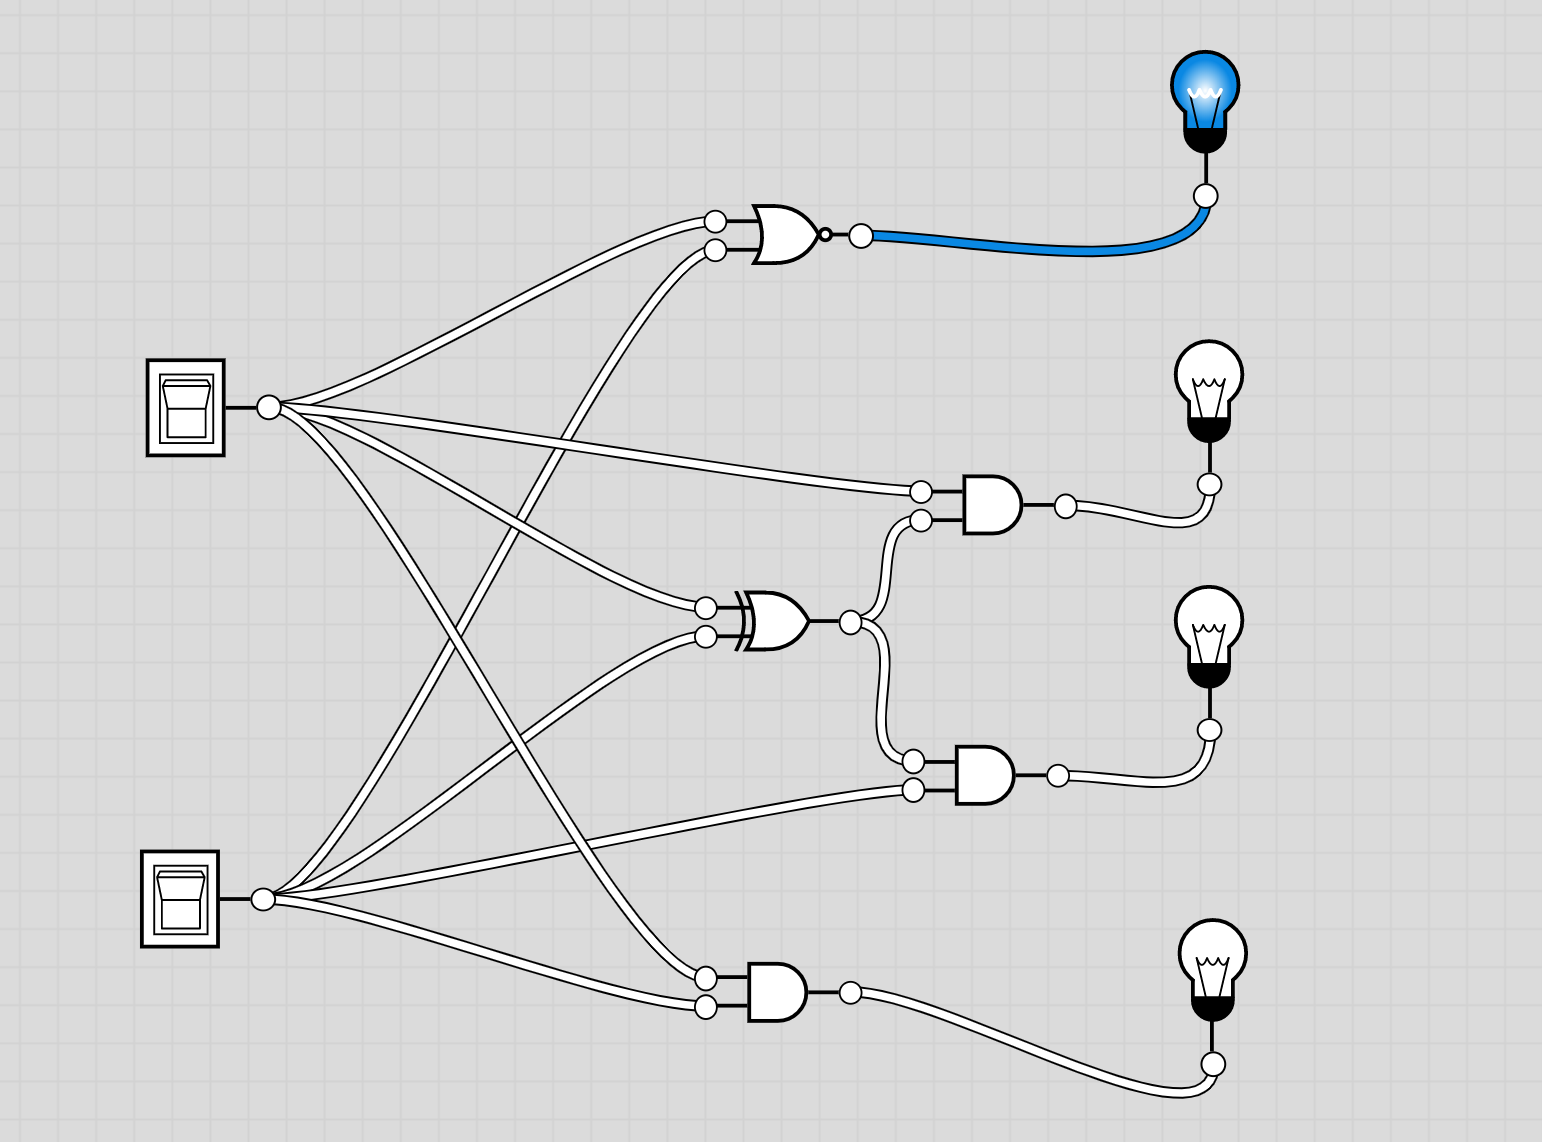
\includegraphics[width=0.3\textwidth]{data/2018-S1-3-1.png}
%     % \caption{Caption}
%     % \label{fig:my_label}
% \end{figure}
